\chapter{Introduction}
\label{chap:introduction}

Anatomy is learned across several representations at once. A student may encounter the same structure as a name in a glossary, a description in a textbook, a labelled region in a figure, and a three-dimensional object whose orientation changes with the viewpoint. Knowing one representation does not automatically make the others easy to interpret. This is particularly clear for structures whose course, laterality, or relation to neighbouring anatomy matters as much as their name. Studies of three-dimensional anatomy resources report benefits for factual and spatial learning in some settings, but they also show that the educational value depends on the task, the learner, and the way the resource is used \parencite{yammine2015,moro2017}.

Conversational software can make this material easier to reach. Instead of searching several chapters for the wording used by an author, a learner can ask a question in ordinary language. That convenience creates a trust problem, however. A fluent answer can be weakly supported, and a message claiming that a 3D model was generated may appear even when no usable file exists. In both cases, the interface can look successful while the underlying evidence is missing.

The prototype studied in this thesis, \systemname{} (titled \emph{Chatbot for Anatomy} in the formal front matter), responds to these problems through two distinct pipelines. One pipeline uses retrieval-augmented generation (\RAG{}) over uploaded anatomy PDFs and returns passages, source information, and optional figures. The other uses the Model Context Protocol (\MCP{}) to resolve a requested structure and invoke a controlled Blender export from Z-Anatomy. They share an application shell, but they are not treated as one undifferentiated chatbot. A document answer is examined against retrieved evidence; a 3D request is accepted only when the toolchain returns an inspectable artefact.

\section{Motivation}
\label{sec:introduction-motivation}

Anatomy teaching has always relied on more than prose. Written explanations are effective for definitions, functions, and causal relationships, whereas diagrams make selected relations visible and manipulable models expose depth and orientation. A learner may remember that the femoral nerve exists yet remain uncertain about its course, or recognise a labelled image without being able to reconstruct the same relationship from another view. Moving between text, image, and space is therefore part of the subject rather than an optional presentation choice.

Three-dimensional visualisation is most useful when the learner would otherwise have to infer depth from a flat image. In their meta-analysis, \textcite{yammine2015} found benefits for factual and spatial outcomes. The finding is encouraging, but it is not an argument for replacing established teaching methods. \textcite{moro2017}, for example, reported comparable assessment performance across virtual-reality, augmented-reality, and tablet conditions while also observing differences in engagement and adverse effects. I therefore treat 3D material in this project as a complementary study aid, not as a substitute for dissection, teaching, or conventional resources.

Natural-language interaction addresses a different difficulty: learners do not always know the terminology used by a source. They may ask for a simpler explanation, compare two structures, or describe a relationship imprecisely. A conversational interface can help with that translation. Its usefulness depends on whether the answer can still be traced back to the uploaded material. If the response draws on broader model knowledge, the user should not be led to believe that the information came from the course PDF.

A similar distinction applies to 3D requests. The useful outcome is not a reassuring sentence but a model that can be opened and inspected. The project was consequently driven by three practical needs: local documents should support traceable answers; figure-related questions should be able to return material from the same corpus; and a named 3D structure should lead to bounded software execution with a verifiable output. Much of the thesis concerns what happened when those apparently simple requirements met the actual implementation.

\section{Problem Statement}
\label{sec:introduction-problem}

Large language models generate text from learned parameters and the context supplied at inference time. Because the output is fluent, a novice may not recognise when a statement is unsupported. In this thesis, hallucination refers to content that lacks support in the relevant evidence or is unfaithful to the supplied source \parencite{ji2023}. The concern is especially serious in anatomy, where a small error in laterality, innervation, or structural relation can change the meaning of an explanation.

Merely uploading a PDF does not give the model dependable access to that document. The application must extract usable content, divide it into passages, retrieve relevant evidence, and include that evidence in the generation step. \RAG{} provides this external-memory pattern \parencite{lewis2020}. It also introduces a chain of possible failures: extraction can omit material, chunking can split an explanation, retrieval can select a related but insufficient passage, and the generator can add details not present in the context.

For a course-oriented assistant, provenance has to survive the full route from ingestion to display. A filename and page number are helpful only when the passage actually supports the nearby claim. Conversely, an answer can be correct in general and still fail the stated task if the uploaded corpus does not contain the supporting information. I therefore distinguish retrieval, evidence sufficiency, synthesis, citation, and abstention throughout the thesis instead of using the broad label ``grounded'' for all of them.

Text retrieval alone also misses questions for which the visual material carries much of the information. Anatomy PDFs contain diagrams, cross-sections, radiological images, and labelled composite figures. A multimodal assistant must retrieve these as separate objects and retain their source context. Text and image quality cannot be collapsed into one judgement: a strong answer can be paired with an irrelevant figure, and a relevant figure cannot rescue an unsupported explanation.

The 3D workflow presents a different kind of failure. A language model can write ``the femur has been exported'' even when no file was created. For this reason, the operation must end in structured tool output and an accessible artefact. \MCP{} provides a host--client--server protocol for discovering and calling tools with defined schemas \parencite{mcp20250618}. The protocol makes the action easier to inspect, but it does not remove the need to resolve the correct structure, run Blender, verify the files, and load the result in the viewer.

The engineering problem addressed here is therefore not simply how to add more modalities to a chatbot. It is how to preserve the right form of evidence for each output. Document answers require passages and source handling. Three-dimensional requests require constrained execution and artefact checks. The final architecture grew out of making that difference explicit.

\section{Research Positioning and Gap}
\label{sec:introduction-gap}

The work sits at the intersection of educational language models, hallucination research, \RAG{}, multimodal retrieval, anatomy visualisation, and tool-using systems. Educational LLM research describes opportunities for explanation and personalised support while also documenting risks involving accuracy, bias, privacy, and over-reliance \parencite{kasneci2023}. Hallucination studies motivate closer attention to evidence \parencite{ji2023}; \RAG{} offers a practical way to condition answers on external documents \parencite{lewis2020}; and anatomy-education studies explain why spatial material may be useful \parencite{yammine2015,moro2017}.

None of these components is claimed as a new method. Nor does the thesis claim that no similar anatomy system exists: the literature review is structured and narrative rather than systematic. The narrower gap is practical and evidential. When one educational interface offers both document-based answers and executable 3D outputs, each result needs a different verification path. This project investigates how that separation can be implemented and how limitations should be reported when parts of the intended design remain incomplete.

The development history is also part of the research contribution. The final system was not specified at the beginning. Dense retrieval, figure extraction, storage, procedural geometry, scene-label search, and direct function calls each exposed a different weakness. Reconstructing those decisions shows why the architecture changed and prevents later chapters from presenting unfinished branches as measured improvements.

\section{Aim and Objectives}
\label{sec:introduction-aim-objectives}

The aim of this thesis is to design, implement, and evaluate a multimodal anatomy learning assistant that answers questions from uploaded educational documents and uses a separate tool-based workflow to create inspectable 3D anatomy artefacts.

The work pursues five objectives:

\begin{enumerate}[label=\textbf{O\arabic*.},leftmargin=*,itemsep=0.25em,topsep=0.35em]
  \item build an anatomy question-answering pipeline that retrieves evidence from uploaded PDFs and exposes its sources;
  \item add figure retrieval for questions that require visual context;
  \item implement an \MCP{}-based workflow that resolves named structures and exports existing anatomy geometry as inspectable artefacts;
  \item define evaluation procedures that keep document evidence separate from 3D execution evidence; and
  \item document unsuccessful approaches, corrections, trade-offs, and unresolved limitations.
\end{enumerate}

These objectives describe a research prototype. They do not imply clinical validation, production readiness, or a demonstrated improvement in student learning.

\section{Research Questions}
\label{sec:introduction-research-questions}

Four research questions guide the study:

\begin{description}[style=nextline,leftmargin=2.2cm,labelwidth=1.6cm,itemsep=0.35em,topsep=0.35em]
  \item[\textbf{RQ1}] How effectively did the evaluated hybrid-preferred document-RAG pipeline retrieve supporting anatomy passages and respect the boundary of the uploaded corpus?

  \item[\textbf{RQ2}] To what extent did the multimodal retrieval component make figure material available, and which limitations were observed in visual relevance and provenance?

  \item[\textbf{RQ3}] How does the MCP-based verification design distinguish a successful 3D artefact export from an unverifiable natural-language success claim?

  \item[\textbf{RQ4}] What design trade-offs and limitations arise in a local-first multimodal anatomy assistant for educational use?
\end{description}

The wording matches the evidence that was available at the end of the project. The primary English evaluation used the hybrid-preferred production route on \codepath{/rag/ask} after hybrid retrieval was connected in commit \texttt{5089fcc}; dense-only search remained only as a fallback, and no matched dense-versus-hybrid ablation was completed. Figure availability was recorded without an expert relevance baseline, so multimodal improvement is not claimed. The MCP path was implemented as a verification design, but the planned comparative runtime study was not completed, so MCP effectiveness is not claimed as an empirical gain. RQ1 and RQ2 therefore concern the document pipeline, RQ3 addresses 3D verification, and RQ4 brings together the engineering consequences of both.

\section{Contributions}
\label{sec:introduction-contributions}

The thesis contributes a prototype and a critical account of its construction. It does not introduce a new foundation model or claim clinical validation.

\begin{enumerate}[label=\textbf{C\arabic*.},leftmargin=*,itemsep=0.35em,topsep=0.35em]
  \item \textbf{Dual-pipeline architecture.} Document question answering and 3D export are offered within one application while retaining separate sources, processing paths, outputs, and success criteria.

  \item \textbf{Multimodal document support.} The document route combines PDF ingestion, hybrid-preferred retrieval (dense, BM25, and phrase candidates with Reciprocal Rank Fusion), source-aware deduplication, type-dependent context limiting, answer generation, and optional figure retrieval. The contribution lies in the integration and examination of these components in the project setting; hybrid superiority over dense-only retrieval is not claimed.

  \item \textbf{Verification-oriented 3D execution.} Natural-language requests are resolved against an anatomy catalogue and passed to bounded \MCP{} tools. A successful response is tied to structured output and an inspectable artefact derived from Z-Anatomy \parencite{zanatomy}. Empirical MCP effectiveness was not measured in a completed runtime workbook.

  \item \textbf{Output-specific evaluation.} Retrieval and citation evidence are kept distinct from catalogue resolution, tool execution, and artefact evidence. The analysis also records where the evaluated runtime differed from earlier design intent, including the move from a hard three-passage cap to question-type-dependent limits and incomplete world-knowledge enforcement on the production schema.

  \item \textbf{Engineering knowledge from iteration.} The thesis explains why several initially reasonable designs were changed and identifies which proposed corrections still lack controlled evidence.
\end{enumerate}

\section{Scope and Non-Goals}
\label{sec:introduction-scope}

The system accepts anatomy PDFs, supports question answering over indexed material, can return extracted figures, and provides a separate route for requesting 3D structures. The evaluation focuses on technical behaviour: request completion, ranking, source and boundary behaviour, figure availability, and the design of verifiable 3D execution.

In this thesis, \emph{local-first} expresses a preference for keeping documents, indexes, anatomy assets, and generated files under the operator's control. It is not a claim that every optional service used during development was offline. The evaluated configuration is reported as it was observed rather than forced into an all-or-nothing definition of locality.

The following matters are outside the study:

\begin{itemize}[itemsep=0.25em,topsep=0.35em]
  \item diagnosis, treatment recommendations, patient management, or medical decision support;
  \item certification of the complete medical accuracy of the source documents or the 3D dataset;
  \item elimination of hallucination or unsupported generation \parencite{ji2023,lewis2020};
  \item exhaustive coverage of every structure in the source assets;
  \item claims about examination performance, retention, or spatial ability without a controlled learner study; and
  \item production-scale certification for security, accessibility, concurrency, or institutional deployment.
\end{itemize}

These boundaries limit the conclusions. Corpus evidence can show where an answer was derived from, and an exported file can show that a tool produced an artefact. Neither finding certifies clinical correctness or educational effectiveness.

\section{High-Level Thesis Concept}
\label{sec:introduction-concept}

\begin{figure}[htbp]
  \centering
  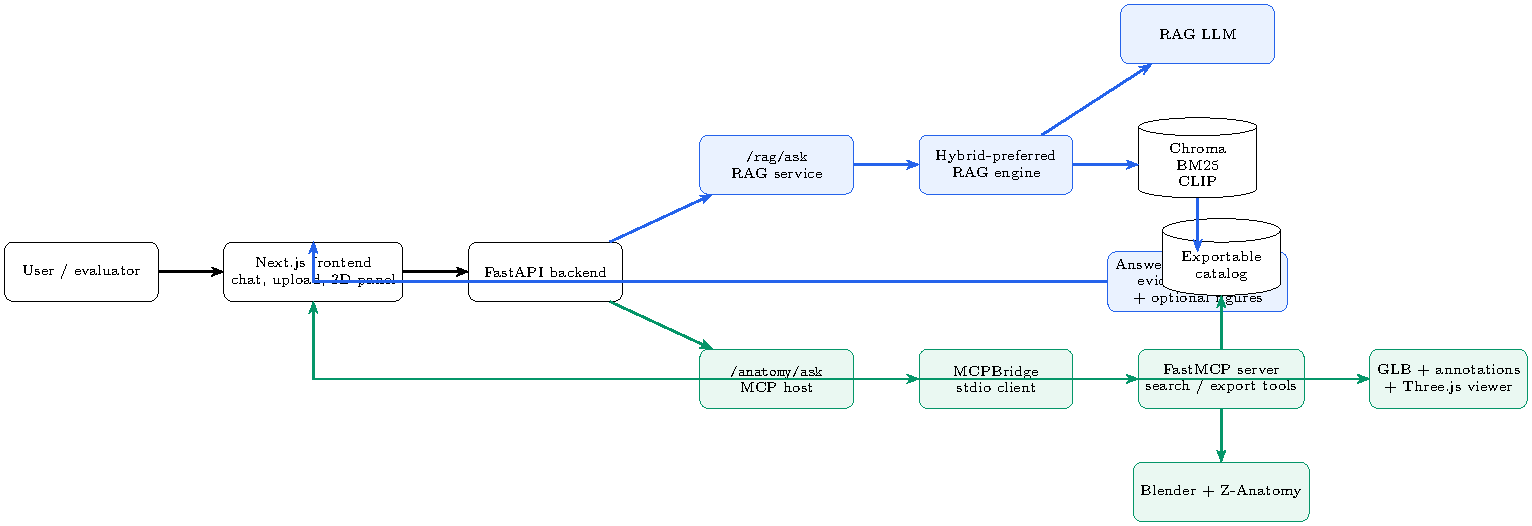
\includegraphics[
    width=\textwidth,
    height=0.64\textheight,
    keepaspectratio
  ]{figures/rendered/dual_pipeline_architecture.pdf}
  \caption{High-level dual-pipeline architecture of the anatomy learning assistant. The document path uses uploaded PDFs with hybrid-preferred retrieval and returns an answer with question-type-capped evidence context and optional figures. The three-dimensional path uses a validated anatomy catalogue and controlled export tools to return an inspectable model artefact.}
  \label{fig:dual-pipeline-intro}
\end{figure}

\Cref{fig:dual-pipeline-intro} shows the division of responsibility. In document mode, passages and optional figures are retrieved before the answer and source metadata are returned. In 3D mode, a structure is resolved against a catalogue and an external export tool is invoked. The evaluation follows the same division: document responses are examined through evidence and citation behaviour, whereas 3D responses require a tool trace and an accessible artefact.

\section{Thesis Structure}
\label{sec:introduction-structure}

\Cref{chap:background} introduces the theoretical and technical foundations. \Cref{chap:methodology} explains the research approach, requirements, constraints, and evidence boundaries. \Cref{chap:evolution} reconstructs the decisions that shaped the prototype, and \cref{chap:implementation} maps the final architecture to the archived code. \Cref{chap:evaluation} describes what was and was not evaluated. Results and limitations are discussed in \cref{chap:results}; \cref{chap:conclusion} then answers the research questions and prioritises the remaining work.
